\section{Réhabilitation et serious games pour la santé}
Comme nous l'avons vu, les serious games sont des outils efficaces pour servir une cause sérieuse par l'intermédiaire du jeu. Ils peuvent aussi être utilisés pour aider à la rééducation fonctionnelle en augmentant la motivation des patients ou à améliorer leur style et hygiène de vie.
		\subsection{De nouvelles modalités pour la thérapie}
Walt Scacchi\cite{Scac11} s'est intéressé à la question et a cherché à connaître quels sont les paramètres importants pour qu'un tel jeu soit efficace et puisse aider en thérapie et réhabilitation. Il a étudié différents types de jeux comme \emph{Quest for the Code}, un jeu pour apprendre aux joueurs à mieux connaître et gérer leur asthme, \emph{Famscape}, un jeu social encourageant à des objectifs de vie sains ou encore \emph{SimHealth}, jeu de simulation d'un système de santé national.

\paragraph{}
Scacchi\cite{Scac11} résume en trois points clefs comment les jeux peuvent aider en thérapie et réhabilitation~:
\begin{enumerate}
	\item \textbf{motivation }: challenge, histoire, compétition. C'est le $\rightarrow $ "\emph{why I start}".
	\item \textbf{soutien} : interface, processus de jeu, conseil du personnage, cohésion multijoueur. C'est le $\rightarrow $ "\emph{why I enjoy playing}".	
	\item \textbf{maintien} : boucles de jeux, modèles d'engagement durables, score, progression, immersion. C'est le $\rightarrow $ "\emph{why I keep playing}".
\end{enumerate}

Il définit aussi quatre domaines d'intervention pour permettre le changement de comportement pour la santé\cite{Scac11}~:
\begin{enumerate}
	\item augmenter activités physiques et performances.
	\item sensibiliser à une bonne gestion de sa santé.
	\item améliorer son hygiène de vie.
	\item proposer des thérapies d'aide.
\end{enumerate}
		
Burke et al\cite{Burk09} ont précisé l'intérêt particulier de la motivation dans les serious games. Selon eux, son facteur principal est le challenge proposé par le jeu. Le niveau de difficulté doit ainsi suivre une courbe croissante pour s'adapter à l'évolution du joueur (figure~\ref{courbe_difficulte}).
\begin{figure}
	\centering
	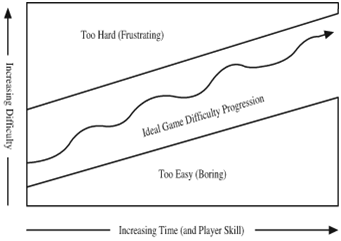
\includegraphics[scale=1]{images/courbe_difficulte.png}
	\caption{Évolution idéale de la difficulté dans un SG [Rabin, 2005]}
	\label{courbe_difficulte}
\end{figure}

Le challenge doit correspondre aux capacités du patient. Au commencement d'un jeu, un joueur va généralement désirer un niveau de jeu faible qui correspond à sa familiarité avec le jeu. Ils proposent pour cela de passer soit par un ajustement manuel de la difficulté soit par une adaptation dynamique des éléments du jeu.

	\subsubsection*{Proposer de nouveaux contrôles}
Se concentrant sur les serious games destinés aux personnes âgées, [Gerling and Masuch, 2011]\cite{Gerl11} déplorent la complexité des périphériques grand public tels que les accessoires de la Wii. \\
Afin d'aider à augmenter la motivation des joueurs, proposer de nouveaux types d'interactions est un enjeu majeur [Gerling and Masuch, 2011].

\paragraph{} Scacchi\cite{Scac11} et [Burk et al]\cite{Burk09} ont ainsi référencé les usages de différents périphériques dans les serious games pour la santé. Ils proposent aussi l'utilisation de périphériques existants dont l'utilisation pourrait se prêter à un usage thérapeutique. \\
On retrouve ainsi~:
\begin{itemize}
	\item Guitare (de Guitar Hero) et batterie (de Rock Band).
	\item Joystick, trackball (boule de commande) et volant haptique.
	\item Contrôleurs avec retour de force : volant de course, vessie pneumatique, etc.
	\item Contrôleurs multi-senseurs : vidéo, IR, accéléromètre, neuro-senseur, électro goniomètre, accessoires de la Wii, etc.
	\item Remote and Nunchuk, Kinect
	\item Contrôleurs multi-articulés, ou 'équipés' : data gloves, GypsyMIDI, MYO, etc.
	\item Joystick d’entraînement chirurgical endoscopique : Simball 4D
\end{itemize}

\begin{figure}
	\begin{minipage}{0.49\linewidth}
		\centering
		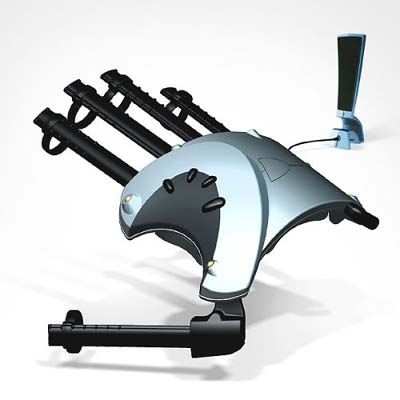
\includegraphics[width=6cm]{images/p5_gloves.jpg}
		\caption{Gants multiarticulés P5~Gloves}
		\label{p5gloves}
	\end{minipage}
	\begin{minipage}{0.49\linewidth}
		\centering
		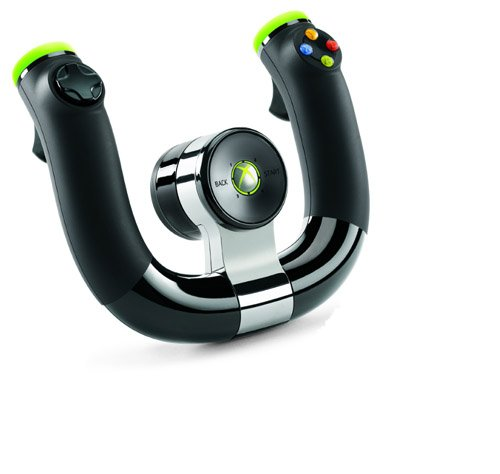
\includegraphics[width=6cm]{images/volant_haptique.jpg}
		\caption{Volant haptique pour xBox 360}
		\label{volant_haptique}
	\end{minipage}
\end{figure}

\paragraph{} L'utilisation de télécommandes Wii ou d'instruments factices pour simuler l'utilisation de vrais instruments est un exemple qui possède un potentiel de rééducation important. De nombreuses possibilités en terme de réhabilitation des bras et des poignets sont envisageables, et possèdent de nombreux atouts~: feedback auditif, feedback visuel, niveau de difficulté ajustable (en fonction de la musique jouée) et motivation importante pour le joueur.

		\subsection{Proposer des jeux adaptés}
Un des principaux problèmes de d'utilisation de jeux pour la santé est celui de l'adaptation du jeu aux capacités du joueur-patient\cite{Flor08}. Ceux-ci sont des joueurs particuliers et les jeux classiques du commerce sont rarement en relation avec leurs capacités.

Gerling et Masuch\cite{Gerl11} déplorent que bien que l'utilisation de jeux vidéo chez les seniors ait des effets positifs sur leur bien-être général, peu de jeux leur sont pleinement accessibles.\\
Il est important de prendre en compte les capacités cognitives et motrices du joueur dans la conception du jeu.

\paragraph{}
S'intéressant à l'utilisation de jeux chez les seniors, ils notent de nombreuses difficultés chez les joueurs joueurs, dues à leur capacités diminuées, à différents niveaux~:
\begin{enumerate}
	\item \textbf{les interfaces} : trop complexes, trop colorées, surchargées d'informations, navigation non intuitive pour des personnes néophytes du jeu vidéo, polices trop petites, trop grande variété de possibilités dans les menus.
	\item \textbf{les contrôleurs} : balance board et Wii Remote facilement pris en main par les joueurs MAIS~:
	\begin{itemize}
		\item Balance : impossibilité de calibrer correctement en position assise, seule position possible pour un certain nombre de personnes. \newline
		$\rightarrow$ repenser la calibration.
		\item  Wii Remote : appuie fréquent sur des boutons (+ et -) de manière involontaire, ce qui a pour effet d'ouvrir une pop-up.\newline
		$\rightarrow$ à modifier pour ne pas prendre en considération les inputs parasites
		\item La combinaison d'inputs haptiques et de boutons est trop complexe, nécessite une synchronisation difficile.
	\end{itemize}
	\item \textbf{le gameplay}:
	\begin{itemize}
		\item Les temps de réaction attendus trop courts ...
		\item … associés à la complexité et multiplicité des options disponibles.\newline
		$\rightarrow$ proposer un gameplay adaptable ou adapté
		\item Performance attendue trop élevée (scoring inadapté) et donc décourageante.\newline
		$\rightarrow$ ajuster le seuil de valeurs pour les feedback
		\item Durée des jeux trop importante et enchaînement trop rapide, ne laisse pas aux joueurs le temps de récupérer, alors qu'ils s'épuisent plus vite.
	\end{itemize}	
\end{enumerate}
Ces problèmes sont d'autant plus importants qu'ils empêchent le joueur de facilement rentrer dans le jeu et peuvent avoir pour effet de faire perdre tout intérêt pour celui rapidement.
\begin{figure}
	\centering
	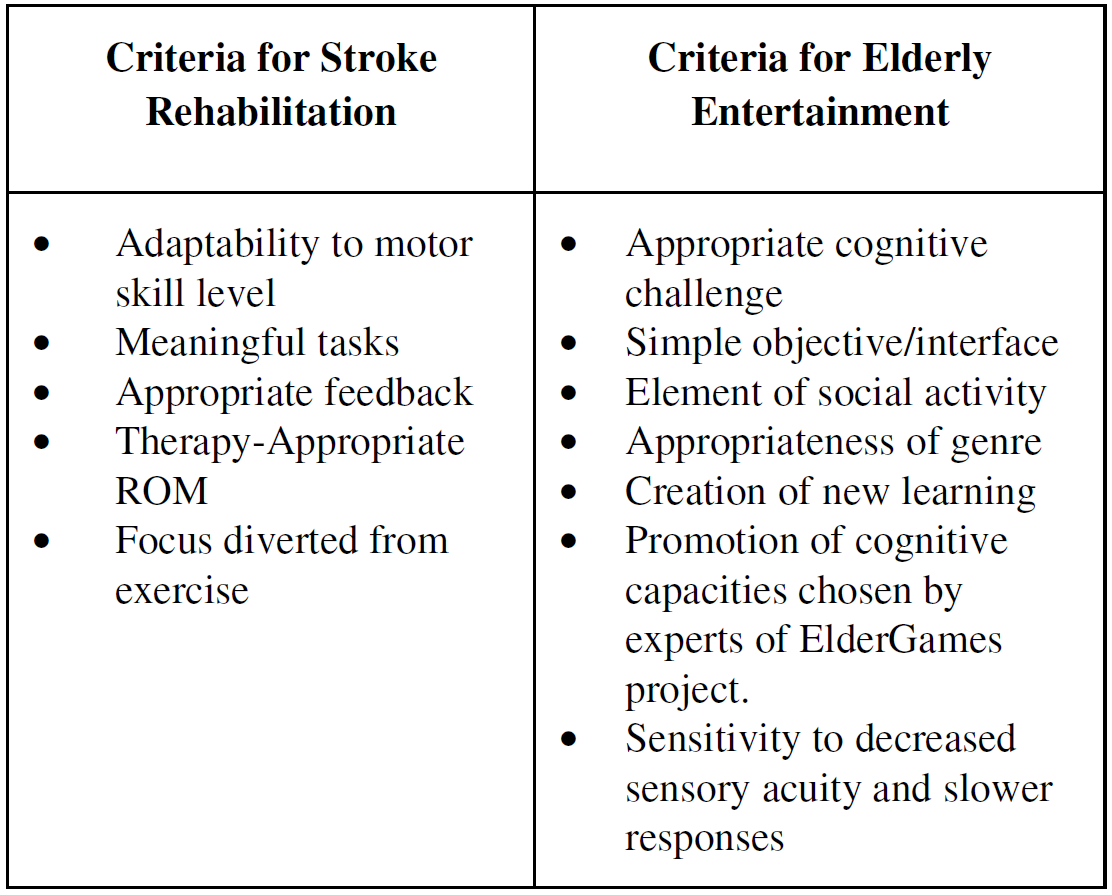
\includegraphics[width=10cm]{images/param_jeux_adaptes.png}
	\caption{Critères à remplir pour proposer un serious game adapté aux personnes âgées et aux personnes hémiplégiques[Flores et al, 2008]\cite{Flor08}}
	\label{param_jeux_adaptes}
\end{figure}

Finalement, [Flores et al, 2008]\cite{Flor08} ont résumé les points importants à prendre dans la conception de serious games adaptés aux personnes âgées et aux joueurs hémiplégiques (figure~\ref{param_jeux_adaptes}).

\paragraph{\emph{Outils d'aide à la conception de SG thérapeutiques}\\}
Partant du même constat du problème de l'adaptation des jeux sérieux pour les patients, Goude, Björk et Rydmark\cite{Goud07} ont choisi d'orienter leur travail vers une aide à la conception de ce type de jeu.

\paragraph{}
Ils définissent des patterns de conceptions de SG thérapeutiques pour permettre aux développeurs de cette jeune industrie (a priori encore peu à l'aise avec la création de ce type de jeu) d'avoir différentes bases de conceptions possédant chacune leurs variations et différences.\\
Ils proposent aussi une taxonomie (figure\ref{taxonomy_conception}) basée sur une ligne directrice de traitements et de soins. 

\begin{figure}
	\centering
	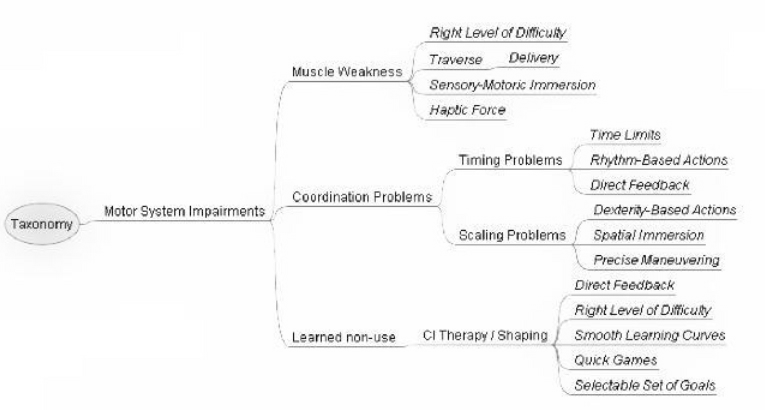
\includegraphics[width=15cm]{images/taxonomy_conception.png}
	\caption{Sous ensemble de la taxonomie proposée par Goude et al\cite{Goud07} sur les troubles moteurs}
	\label{taxonomy_conception}
\end{figure}

\paragraph{}Ils font ensuite la liaison entre les patterns et cette taxonomie. L'exploration théorique des manques dans ce mapping a permis de découvrir de nouveaux schémas de conception. On notera qu'une vingtaine jeux basés sur cette taxonomie a été créé à l'écriture de l'article, menant à la création de nouveaux patterns afin de permettre la création de nouveaux types de jeux et de plus de variations. Ces variations fournissent une gamme d'activités qui peut être utilisée pour personnaliser la session de rééducation, puisque les patterns, avec toutes les variations, possèdent une tache spécifique (de la taxonomie de soin) mappée avec celui ci.

\paragraph{}On notera enfin l'importance de la communication entre les développeurs et les médecins. L'association entre patterns et traitements doit être vérifiée, et la taxonomie étendue (seul un sous-ensemble des symptômes d'une attaque est actuellement considéré).